% Template for ICIP-2013 paper; to be used with:
%          spconf.sty  - ICASSP/ICIP LaTeX style file, and
%          IEEEbib.bst - IEEE bibliography style file.
% --------------------------------------------------------------------------
\documentclass{article}
\usepackage{spconf,amsmath,graphicx}
% 한글 패키지
\usepackage{kotex}
\usepackage[unicode, hidelinks]{hyperref}
\usepackage{subfigure}

\usepackage{gensymb}


% *** MATH PACKAGES ***
%
\DeclareMathOperator*{\argmin}{argmin}
\usepackage{amsfonts}

% Example definitions.
% --------------------
\def\x{{\mathbf x}}
\def\L{{\cal L}}

% Title.
% ------
\title{A Novel Filtering Approach for Robust and Fast Keypoint Matching in Mobile Environment}
%
% Single address.
% ---------------
% \name{Jonghoon Seo$^{1}$, Seungho Chae$^{2}$, Yoonsik Yang$^{2}$, Tack-Don Han \thanks{Thanks to KIST and NFS for funding.}}
% \address{	Software Platform R\&D Lab.\\ LG Electronics Advanced Research Institute\\ 19 Yangjae-daero 11 gil, Seocho-gu, Seoul 137-893, Kore}

% For example:
% ------------
%\address{School\\
%	Department\\
%	Address}
%
% Two addresses (uncomment and modify for two-address case).
% ----------------------------------------------------------
\twoauthors
 {Jonghoon Seo}
	{LG Electronics\\
	Software Platform R\&D Lab.\\
	19 Yangjae-daero 11 gil, Seoul, Korea}
 {Seungho Chae, Yoonsik Yang, Tack-Don Han\sthanks{This }}
	{Yonsei University\\
	Department of Computer Science\\
	50 Yonsei-ro, Seoul, Korea}

 %
\begin{document}
%\ninept
%
\maketitle
%
\begin{abstract}
Local keypoint matching method is widely used because it can provide robust to environment change and occlusion. In this paper, we propose a novel keypoint filtering approach, which accomplish not only fast, but also robust and reliable matching. The proposed approach, in offline learning phase, evaluates detected keypoints with proposed criteria and stores only high-distinguishable keypoints. This approach reduces the number of stored keypoints, also reduces false matching rate and attains fast and robust matching quality. We evaluated this approach in mobile augmented reality application, and proved the proposed approach is effective in terms of both matching speed and quality.

% 로컬 키포인트 매칭 방법은 조명 변화나 가려짐 등에서도 강인한 매칭 성능을 제공하기 때문에 다양한 이미지 매칭 어플리케이션에서 사용되고 있다. 본 논문에서는 빠를 뿐만 아니라 강인한 인식 성능을 제공하기 위하여 키포인트 필터링 방법을 제안한다. 제안하는 방법은 offline learning 단계에서 추출된 키포인트들을 평가하여 구분이 잘 되는 점들만을 저장한다. 이를 통하여 저장되는 키포인트의 개수를 줄이면서도 false matching을 줄여 강인한 인식 성능을 얻을 수 있도록 하였다. 모바일 증강현실 어플리케이션에서 실험결과 제안하는 방법을 적용함으로써 인식 속도가 빨라질 뿐만 아니라, 매칭의 퀄리티도 높아지는 것을 확인할 수 있ㄷ었다. 이러한 방법을 통해 모바일 및 임베디드 컴퓨팅 환경에서 더 빠르고 강인한 인식 성능을 제공할 수 있다.

\end{abstract}
%
\begin{keywords}
Keypoint filtering, Keypoint matching, Feature selection, Keypoint saliency, Image matching
\end{keywords}
%
%!TEX root = ../icip_jseo.tex
% -*- root: ../icip_jseo.tex -*-

\section{Introduction}
\label{sec:intro}

Image matching is a fundamental problem in a variety of computer vision applications, including object recognition\cite{nister_scalable_2006}, panorama stitching\cite{brown_recognising_2003}, and augmented reality\cite{wagner_multiple_2009}. To accomplish image matching, keypoint-based local matching is widely used, since it can provide relatively high matching quality against severe occlusion and do not require segmentation for regions of interest. Also, recent work has concentrated on making invariant to image transformation with low computing power\cite{carrera_robust_2007,mikolajczyk_performance_2005}.

% To enhance the image matching quality in various environments, many related techniques have been proposed, such as keypoint-based local matching, histogram-based global matching\cite{le_improving_2013}, color-based matching\cite{mehtre_color_1995}, and template-based matching\cite{korman_fast-match:_2013}, etc. Among them, keypoint detection and matching has created great interest 

The overall flowchart of keypoint matching and recognition is shown in Fig. \ref{fig:on_offline_process}. This procedure can be divided into two main phases: offline learning (or training) and online testing procedure. Offline learning is a prerequisite to online matching process. In offline learning phase, a set of reference images to be recognized is analyzed and stored a set of descriptors in a database. In online testing phase, a newly captured image is analyzed and compared with the reference images in the database to find a nearest reference image. 
% In each phase, common procedures for matching are keypoint detection, description, and matching. To analyze training images, at first, keypoints are detected from the images. Then, from those keypoints, local textures are analyzed and described. In this procedure, to provide robustness against rotation, scale, perspective transform, descriptors are constructed. Then, to be used in online phase, efficient matching structures, as databases, are constructed, such as partitioning trees\cite{arya_optimal_1998,beis_shape_1997}, hashing\cite{salakhutdinov_semantic_2009,lv_multi-probe_2007}. In the online matching phase, the database is used to find the most similar corresponding keypoints pair with a given query image. To find the most similar keypoint pairs, with given a query image, keypoints are detected, detected keypoints are described about local texture, and compared with the preconstructed database.

\begin{figure}[hb!]
\centering
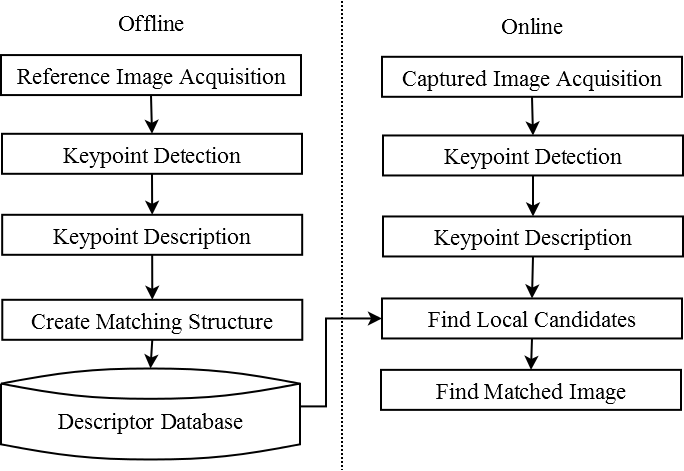
\includegraphics[width=1.0\columnwidth]{1_introduction/process}
\caption{Overall process of conventional keypoint-based matching}
\label{fig:on_offline_process}
\end{figure}

Conventional keypoint matching methods stores almost every keypoints which are detected by keypoint detection process. Keypoint detection processes are designed to extract repeatable keypoints and robust against arbitrary image transformation. Then, detected keypoints are independent to the follow matching procedures, and do not reflect quality of descriptors. Therefore, as seen Fig. \ref{fig:example_of_bad_features}, some keypoints are not distinguishable, and they tend to cause inter-keypoint confusion and miss matching. Also, those detected keypoints are stored in database and are compared with keypoints in query images in every frame while matching. Then, it decreases the speed of matching. To overcome these problem, in offline learning procedure, detected keypoints are evaluated with respect to proposed matching quality criteria and filtered by the goodness score. With this filtering method, only a small subset of keypoints is stored in the database. Accordingly, it provides more improved matching performance with faster matching speed.

\begin{figure}[ht!]
\centering

\includegraphics[width=0.5\columnwidth]{1_introduction/checkerboard}
\caption{Example of high repeatable but poor distinguishable keypoints. Conventional keypoint matching systems do not consider the discriminability of keypoints, so these keypoints usually stored and negatively affected matching.}
\label{fig:example_of_bad_features}
\end{figure}

Especially, mobile devices still have insufficient computing power and limited memory compared to desktop, so there is an urgent need of effective processing methods for image matching. However, conventional keypoint matching approaches stored redundant keypoints into database, and these redundant keypoints may are compared in every frame. So, matching speed will be decreased and this causes problem in the mobile computing devices. On the other hand, the proposed method removes redundant keypoints in the database, it reduces the number of comparisons while matching and increase matching speed even in the mobile computing environment.

This paper is structured as follows: In Chapter 2, we discuss literature on light-weight keypoint-matching algorithms. Chapter 3 describes the proposed keypoint score function. In Chapter 4, we executed experiments to prove the proposed keypoint filtering method in various algorithms and compared over several evaluation metrics. Finally, Chapter 5 presents the conclusion.

%!TEX root = ../icip_jseo.tex
% -*- root: ../icip_jseo.tex -*-


\section{Related Works}
\label{sec:relworks}

%하지만 이러한 feature matching 기반의 markerless AR 알고리즘은 연산량이 많기 때문에 mobile phone과 같은 smart space 환경에서는 자연스러운 동작이 어렵다. 이를 극복하기 위하여 다양한 경량화 알고리즘들이 제안되고 있다. 특히, 그림 xxx\todo{매칭 속도 비교 새 버전 입력}에서 보듯이 전체적인 연산 성능에 큰 영향을 미치는 단계인 feature description과 matching 단계에 대한 속도 향상이 많이 이루어지고 있다.



%먼저, keypoint descriptor는 기존의 SIFT\cite{lowe_distinctive_2004}나 SURF\cite{bay_speeded-up_2008}와 같은 vector value-based description 방법은 높은 인식율을 제공해 주었지만, orientation과 scale 등의 distortion에 robust한 descriptor를 생성하기 위하여 복잡한 연산을 수행하여야 하기 때문에 연산이 복잡하게 수행되었다. 따라서 최근에는 BRIEF\cite{calonder_brief:_2010}, ORB\cite{rublee_orb:_2011}, BRISK\cite{leutenegger_brisk:_2011}, FREAK\cite{alahi_freak:_2012}과 같은 다양한 Binary value-based descriptor들이 개발되고 있다. 이러한 Binary descriptor들은 그림 xxx\todo{binary desciprot 패치 }와 같이 특징점을 중심으로 다양한 형태의 패턴을 이용하여 두 점 사이의 밝기 값을 비교하여 binary code로 표현하는 방법이다. 단순 비교 연산만으로 descriptor를 계산하기 때문에 vector-based descriptor에 비하여 연산 속도가 상당히 빠르며, 최근에는 생성 패턴을 기준으로 orientation이나 scale 등을 normalize 하기 때문에 다양한 distortion에서도 상당히 강인한 성능을 보여주고 있다. 특히 smart space와 같이 제한된 성능의 환경에서는 vector-value descriptor 기반의 복잡한 연산 보다는 단순 비교연산만으로도 처리가 가능한 binary descriptor를 사용하는 연구가 많아지고 있다. 

In spite of robust matching quality, keypoint-based local matching requires a large amount of computation, especially in mobile computing environment. To overcome this limitation, various lightweight algorithms are proposed. At first, in the study of keypoint descriptors, the vector-value based description methods such as SIFT\cite{lowe_distinctive_2004} or SURF\cite{bay_speeded-up_2008} provide robust recognition quality, but complex computation is required to calculate descriptors. In recent years, variant binary-value based descriptors, such as  BRIEF\cite{calonder_brief:_2010}, ORB\cite{rublee_orb:_2011}, BRISK\cite{leutenegger_brisk:_2011}, FREAK\cite{alahi_freak:_2012}, are proposed. These binary descriptors compare the brightness values with focus on the keypoints as shown in Figure \ref{fig:markerless_binary_patterns} by using a wide range of form patterns and express the results in binary codes. Since descriptors are computed only by a simple comparison computation, its computational speed is significantly faster than vector-based descriptors. Moreover, since the orientation and scale are normalized on the basis of generation patterns, they show significantly robust performance against a wide range of distortion. In particular, studies using the binary descriptors that can be processed by simple comparison computation rather than complex vector-value descriptor based computation are increasing in the environment of limited performance such as a mobile computing.  

\begin{figure}[hb!]
  \centering     %%% not \center
    \subfigure[BRISK\cite{leutenegger_brisk:_2011} Sampling Pattern]{\label{fig:markerless_brisk}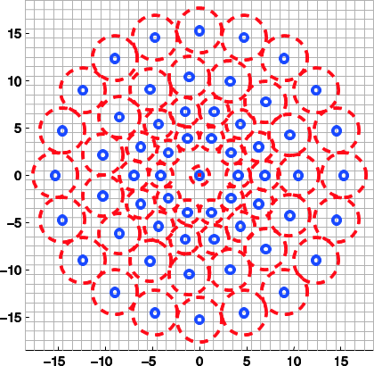
\includegraphics[width=0.48\columnwidth]{2_relworks/brisk}}
    \hfill
    \subfigure[FREAK\cite{alahi_freak:_2012} Sampling Pattern]{\label{fig:markerless_freak}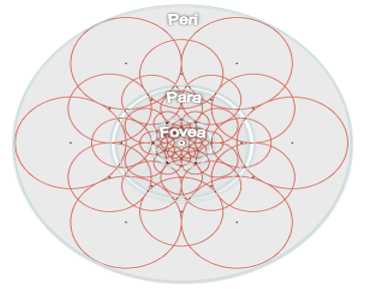
\includegraphics[width=0.48\columnwidth]{2_relworks/freak}}
  \caption{Sampling Patterns of Binary Descriptors}
    \label{fig:markerless_binary_patterns}
\end{figure}


%다음 방법은 matching data structure를 효율적으로 설계하여 nearest neighbor match를 빠르게 수행하도록 하고 있다. 기존의 brute force matching 방법은 query image의 모든 keypoint들을  reference image의 모든 keypoint들과 비교하는 방식으로 가장 속도가 오래 걸리지만, 가장 정확한 nearest neighbor를 검출할 수 있다는 장점이 있다. 이를 개선하기 위하여 다양한 tree 기반의 approximated nearest neighbor 검출 기법들이 사용된다. \cite{beis_shape_1997}에서는 kD tree 기반의 approximation 방법이 제안되었다. 이 방법은 특징의 차원이 비교적 적은 SIFT나 SURF와 같은  vector-value description 방식에서는 좋은 성능을 보여주지만, 최근에 사용되는 binary descriptor에서는 dimension이 높아 성능향상을 기대하기 어렵다는 문제가 있다. LSH\cite{gionis_similarity_1999}와 같은 Hashing 기반의 structure를 이용하여 matching 을 가속화하는 방법도 제안되었다\cite{rublee_orb:_2011}. 이러한 방법은 offline training 단계에서 적절히 특징점들이 고르게 분포하도록 적절한 hash function set을 구성하는 것이 중요하다. 또한, Random Forest\cite{lepetit_keypoint_2006} 또는 Random Fern \cite{ozuysal_fast_2010}은 Binary Description 방식을 Tree 구조 또는 List 구조에 적용하여 matching structure를 구성하였다. 이러한 매칭 방식들은 인식의 속도를 향상시키고, 좀 더 정확한 approximation 값을 얻기 위하여 일반적으로 offline training 단계에서 계산된 descriptor들을 이용하여 추가의 연산을 적용하여 효율적인 matching structure를 생성한다. 하지만, 이러한 방법들을 사용한 추가적인 구조체가 상당히 복잡하고 용량이 크기 때문에 모바일 환경에서 사용하기에 매칭 구조체가 과도하게 무거워진다는 문제점이 존재한다. 또한, detected keypoint의 성질에 대한 고려가 없기 때문에 detected keypoint set이 분류가 어려운 set 일 경우에는 성능 저하가 크게 된다는 한계가 존재한다. 따라서 본 학위논문에서는 이러한 방법을 해결하기 위하여 Keypoint Filtering 기반의 향상된 매칭 방법을 제안한다.

The other researches accelerates nearest neighbor matching with designing an efficient matching data structure. The conventional brute force matching compares all the keypoints of query images with all the keypoints of reference images, so it shows the slowest, but has the advantage of being able to detect the most accurate nearest neighbors. kD tree based approximation method is proposed in \cite{beis_shape_1997}. This method shows good performance in the vector-value descriptor method such as SIFT or SURF with relatively low dimension of features but the improvement of its performance is unlikely to be achieved in the latest binary descriptor with high dimension. A method enabling it to accelerate matching using Hashing based structure in LSH\cite{gionis_similarity_1999} was proposed\cite{rublee_orb:_2011}. As for this method, it is critical to compose appropriate hash function set to distribute the keypoints points evenly in the offline training phase. In addition, 'Random Forest\cite{lepetit_keypoint_2006}' or 'Random Fern\cite{ozuysal_fast_2010}' composed a matching structure by applying a binary description method to the tree structure or list structure. To increase the recognition speed and obtain more accurate approximation values, these matching methods generate efficient matching structure by way of the application of supplementary computation using the descriptors computed in the offline training phase. However, since the supplementary structure that uses this method is complex and large, its the matching structure is too heavy to use in a mobile environment. Moreover, since the properties of the detected keypoints are not taken into consideration, the set for which it is difficult to classify the detected keypoints may lead to performance degradation. To solve this problem, this dissertation proposes a keypoints filtering based matching methods.  

%!TEX root = ../icip_jseo.tex
% -*- root: ../icip_jseo.tex -*-

\section{Proposed Method}
\label{sec:proposed}


%제안하는 방법은 detect된 특징점을 분석하여 인식에 좋은 정도를 측정함으로써 좋은 특징점만을 filtering 한다. 이를 위하여 좋은 특징점을 정의하였다.

The proposed filtering method stores only good keypoints by analyzing the characteristics of detected keypoints and measuring the degree of effectiveness for image matching. 

There are several factors which good keypoints should follows:

%첫 번째 인식에 좋은 특징점의 조건은 대상 영상이 다양하게 변화되는 환경에서도 안정적으로 특징점으로 검출되어야 한다는 점이다. 실제 온라인 매칭 과정에서 입력되는 카메라 영상에는 인식하고자 하는 대상 영상이 회전이나 크기, perspective, 노이즈, 조명 등의 다양한 형태의 변환이 적용되어 있다. 인식에 좋은 특징점은 이러한 변환된 영상에서도 안정적으로 특징점이 검출이 됨으로써 Descriptor를 생성할 수 있도록 하는 점이어야 한다.
\textit{Repeatability}: Good keypoints need to be stably detected even in various environment. In actual matching environments, a wide range of transformed image degradation may occurred, such as the rotation, size, noise and lighting of the targeted images. The good keypoints have to be stably extracted against those transformation.

%이러한 안정적 특징점 검출은 Repeatability Score로 측정이 가능하다. Repeatability는 아래 그림과 같이 전체 변환된 영상의 개수 대비 변환된 영상에서 키포인트가 변환되어 존재하는 경우의 비율로 계산된다.
The detection of stable keypoints can be measured by \textit{Repeatability} condition. \textit{Repeatability} is calculated by the ratio between the total number of synthesized images and the number of cases where the transformed keypoints are existent in the synthesized images.


\begin{equation}
p_{rep}(p_i) = \frac{n_i^{overlap}}{N}
\end{equation}

% 여기에서 $n_i^{overlap}$는 변환된 영상($T_t(I)$)의 키포인트 집합($K_t'$)에 키포인트($p_i$)가 변환된 점이 존재($T(p_i)\in K_t'$)하는 횟수로 계산되며, $N$은 총 변환된 영상의 개수로 모든 키포인트가 동일한 값을 가지게 된다.

\noindent
where $p_{rep}(p_i)$ represents repeatability score of given point $p_i$, $n_i^{overlap}$ is calculated by the frequency of the existence of transformed keypoint($p_i$) in the set of keypoints($T(p_i)\in K_t'$) of synthesized images $T_t(I)$; $N$ is the total number of synthesized images ; and all keypoints have single value. 

%두 번째 인식에 좋은 특징점 집합의 조건은 해당 키포인트가 변화된 영상에서 만들어진 descriptor와의 매치가 실패가 적어야 한다(Similarity)는 점이다.
%이는 해당 특징점의 Sensitivity(True Positive Rate)와 연관이 있다. Reference 영상의 어떤 특징점($p_i$)에 대하여 학습 과정에서 다양하게 변환된 영상($T_t(I)$)에서의 모든 키포인트 집합($K_t'$)의 Descriptor 사이의 매칭을 계산하여 해당 특징점에 대한 Genuine 분포와 Impostor 분포를 계산할 수 있다. 이 때, 해당 키포인트가 변화된 영상에서의 Descriptor와의 매치가 실패가 적기 위해서는, Genuine 분포가 매치 임계 거리(Match Distance Threshold)에서부터 충분히 떨어져 작은 값을 가져야 한다. 이를 위하여 Genuine 분포의 평균을 이용하여 이를 측정하였다. 식 \ref{eq:similarity}에서 보는 것과 같이, Genuine 분포가 작을 수록 좋은 특징점이기 때문에 genuine 분포의 평균을 normalize 하여 1에서 뺌으로써 평가 함수를 계산하였다.

\textit{Similarity}: Good keypoints need to be well-matched with identical keypoints even though targeted images change in various ways. With regard to a certain keypoint($p_i$) of reference images, genuine distribution' and imposter distribution' for the corresponding keypoint can be measured by calculating the matching between the descriptors of all the sets of keypoints($p_i$) in images($T_t(I)$) transformed in various ways  during the training process. At this time, to reduce the failure in matching the corresponding keypoints and the descriptors in the transformed images, the genuine distribution needs to have small value, being far enough away from match distance threshold. To this effect, it was measured using the mean of genuine distribution. As shown in Equation \eqref{eq:similarity}, the keypoints with the decreasing the genuine distribution are better, so the evaluation function was calculated by normalizing the mean of the genuine distribution and subtracting its value from 1.  

\begin{equation} \label{eq:similarity}
p_{sim}(p_i) = 1 - \frac{\mu_{gen,i} - \min_i \mu_{gen,i}}{\max_i \mu_{gen, i} - \min_i \mu_{gen,i}}
\end{equation}	
where $p_{sim}(p_i)$ represents similarity score of given point $p_i$, $\mu_{gen, i}$ represents mean of genuine distribution of give point $p_i$. 

%세 번째 조건은 학습된 특징점이 자신과 다른 특징점과는 매치가 이루어지지 않아야 한다(Separability)는 점이다. 이는 각 특징점의 Impostor 분포와 관련이 있다. 다양하게 변화된 영상에서 추출된 특징점 중 자기 자신이 변환된 특징점이 아닌 다른 특징점들과의 매칭 분포를 Impostor 분포라 한다. 어떤 특징점이 자신 이외의 다른 키포인트와 낮은 매칭 성공률을 보여주기 위해서는 Genuine 분포와 Impostor 분포가 잘 구분이 되어야 한다.
%이를 위하여 본 논문에서는 Fisher's Discriminant Ratio\cite{fisher_use_1936}를 이용하였다. 이는 1-dimensional, two class problem에서 sample의 평균과 분산에 의하여 두 클래스 사이의 거리를 측정하는 방식이다. 두 번째 Similarity 조건에 의하여 Genuine 분포가 충분히 작음이 보장이 되었기 때문에 Impostor의 분포가 Genuine 분포에 비하여 충분히 떨어져 있다면 Impostor 분포에 존재하는 특징점들과는 매치가 이루어지지 않음이 보장된다. separability 값 역시 수식 \ref{eq:norm_separability}과 같이 normalize 과정이 필요하다.

\textit{Separability}: The trained keypoints and other keypoints shall not be matched, which is associated with the imposter distribution of each keypoint. Of the keypoints extracted from the images converted in various images, the distribution of the matching with other keypoints rather than the converted keypoints themselves are referred to as imposter distribution. Thus for a specific keypoint to show the low success rate of matching with other keypoints rather than themselves, in is necessary that the genuine distribution and imposter distribution are well classified. To this effect, in this paper, \textit{Fisher's Discriminant Ratio\cite{fisher_use_1936}} was used. It measures the distance between two classes by the mean and distribution of sample in 1-dimensional, two class problems. Since the second Similarity condition ensures the genuine distribution is small enough, the nonexistence of the matching with the keypoints in the imposter distribution is ensured if the importer distribution is far enough away compared with the genuine distribution. Separability value also requires the normalization process as shown in equation \eqref{eq:norm_separability}.  


\begin{equation}
FDR(p_i) = \frac{(\mu_{gen,i} - \mu_{imp, i})^2}{\sigma_{gen, i}^2 + \sigma_{imp, i}^2}
\end{equation}
\begin{equation}\label{eq:norm_separability}
p_{sep}(p_i) = \frac{FDR(p_i) - \min_i {FDR(p_i)}}{\max_{i} {s_i}}
\end{equation}	
where $p_{sep}(p_i)$ represents similarity score of given point $p_i$, $\mu_{gen, i}, \mu_{imp, i}$ represent mean of genuine and impostor distribution of give point $p_i$, respectively. $\sigma_{gen,i}, \sigma_{imp, i}$ represent standard deviation of genuine and impostor distribution, respectively.


%이렇게 계산된 세가지 criteria를 이용하여 각 특징점의 score function을 정의할 수 있다. 세 조건은 종속이므로 식 \ref{eq:score_function}와 같이 정의된다.

The score functions of each keypoint can be defined using 3 criteria calculated as above. The 3 conditions are dependent, so can be defined as shown in Equation \eqref{eq:score_function}. 

\begin{equation}\label{eq:score_function}
gf(p_i) = p_{rep}(p_i)p_{sim}(p_i)p_{sep}(p_i)
\end{equation} 



% \subsubsection{}
%%%%% 시간이 되면 실험 부분을 추가하자 %%%%%


%!TEX root = ../icip_jseo.tex
% -*- root: ../icip_jseo.tex -*-


\section{Experiments}

% 앞에서 제안한 특징점 Filtering 알고리즘을 이용하여 학습을 수행하였을 때 인식 성능의 개선을 측정하였다. 

% 실험 영상은, 서울시 가이드 지도 팜플릿 영상 16장을 선택하여 사용되었다. 이러한 영상을 rotation($0.5\sim2.0$배, 0.1배 간격), scale($0\degree\sim360\degree$, $10\degree$ 간격), blur(Gaussian blur, $r=0,3,5,7$pixels) 등의 변형(deformed)한 영상 32,256장 중 random sampling하여 train images 16,114장, test images 16,142장을 선택하였다.
% 먼저 train images에서 특징점들을 검출(detect)하고, detected keypoint 들을 이용하여 앞의 정의된 Score function($gf(p_i)$)을 계산하였다. 

In this chapter, we present several experiments that demonstrate the effectiveness of the proposed method. As for the experimental images, 16 images of Seoul Guide Map Pamphlet was selected. These images were deformed by way of rotating($0.5\sim2.0$-folds, at the interval of 0.1-fold) scaling (($0\degree\sim360\degree$, at the interval of $10\degree$ intervals) and blurring (Gaussian blur, $r = 0,3,5,7$ pixels). As a result, 32,256 images were obtained. Of them, 16,114 training images and 16,142 test images were selected at random. With training images, we detected keypoints and calculated the score function($gf(p_i)$). Then, we stored filtered keypoints and calculated nearest neighbor with test images.

At first, to prove the proposed algorithm can enhance recognition performance, we conducted a comparison experiment(see, Fig. \ref{fig:comparison_agast_freak}). Keypoints are detected with AGAST\cite{mair_adaptive_2010} detector and described with FREAK\cite{alahi_freak:_2012} descriptor. The figure shows comparison among top 50 keypoints based on the proposed score function(\textit{Proposed}), 50 keypoints filtered randomly(\textit{Random}), top 50 keypoints based on the corner response function(\textit{C.R.F.}), and non-filtered $3,000$ keypoints set(\textit{Full}). The figure shows that the proposed approach generates the most robust matching performance.

\begin{figure}[ht!]
\centering
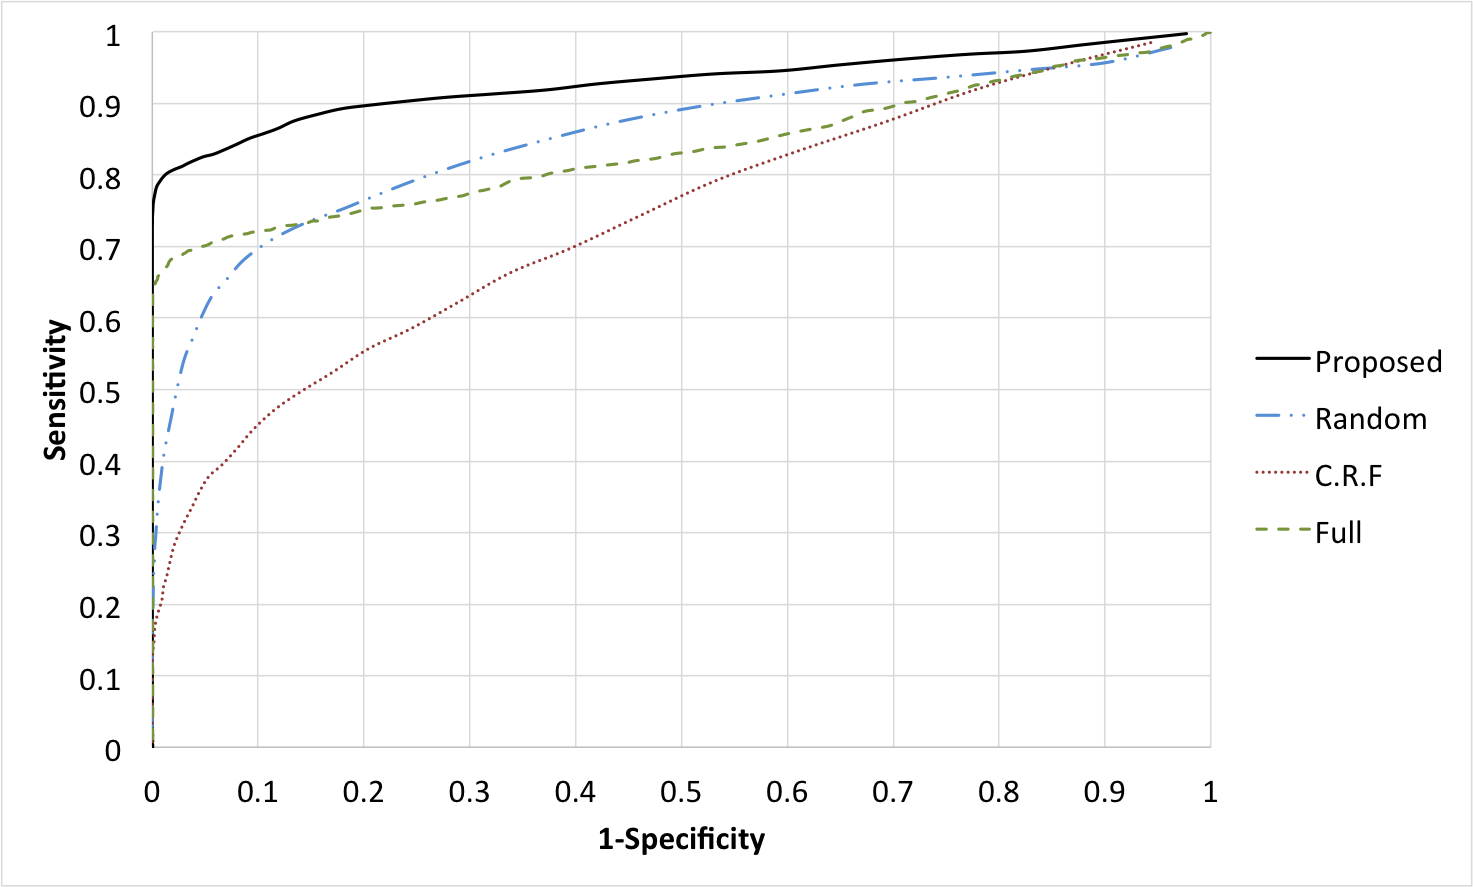
\includegraphics[width=1.0\columnwidth]{4_experiments/comparison_agast_freak}
\caption{ROC curve comparison between proposed filtering function and other methods}
\label{fig:comparison_agast_freak}
\end{figure}

At second, to prove the proposed approach works among several algorithm suits, we performed the comparison tests with changing detection and description algorithms(see, Fig. \ref{algorithm_comparison}). These figures show the proposed method generates robust matching performance even though the algorithm is changed.

\begin{figure}[hb!]
  \centering     %%% not \center
    \subfigure[AGAST detector and BRISK descriptor]{\label{fig:agast_brisk}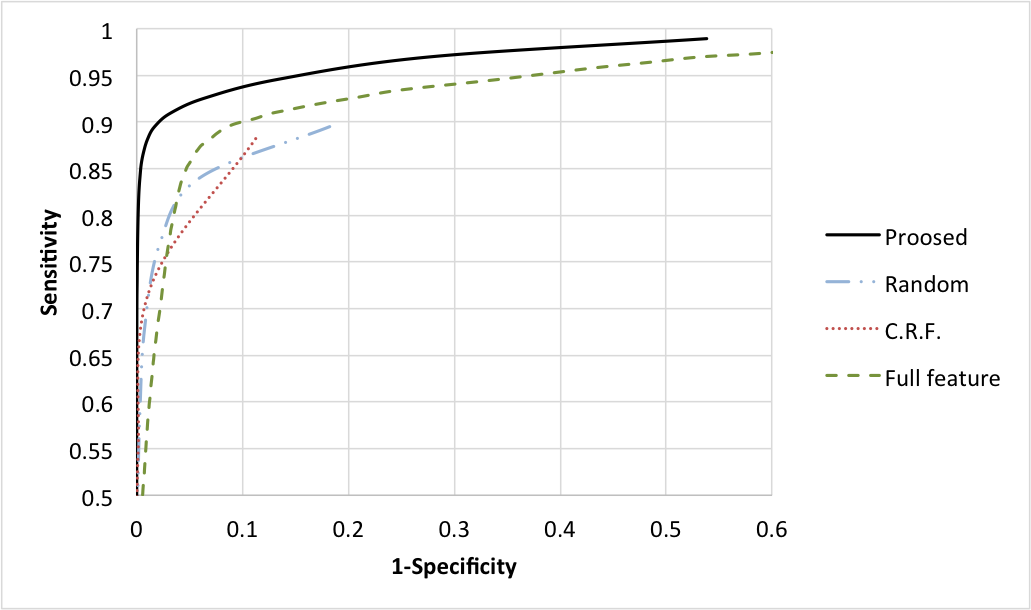
\includegraphics[width=1.0\columnwidth]{4_experiments/agast_brisk}}
    \\
    \subfigure[SURF detector and FREAK descriptor]{\label{fig:surf_freak}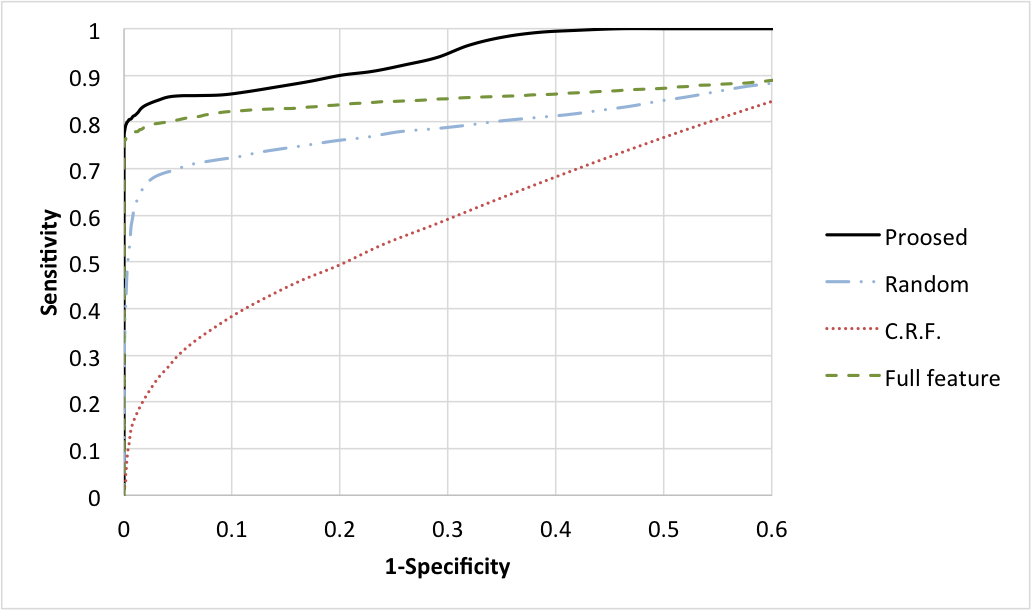
\includegraphics[width=1.0\columnwidth]{4_experiments/surf_freak}}
  \caption{ROC curve comparison between different algorithm sutirs}
    \label{fig:algorithm_comparison}
\end{figure}

%특징점 데이터베이스는 Score function을 고려하지 않은 전체 특징점 집합($K_{all}, n(K_{all}) = 3000$)과, Score function에서 상위 50개, 100개, 300개, 500개 특징점들만 filtering 하여 구성한 특징점 집합($K_{50}, K_{100}, K_{300}, K_{500}$)으로 구성되었다. 

The last experiment is performed to calculate the optimal number of keypoints. The experiment is performed among non-filtered 3,000 keypoints set($K_{all}$), top 500, 300, 100, 50 keypoints subsets($K_{500, 300, 100, 50}$). As shown Fig. \ref{fig:markerless_roc}, the result showed slight degradation of recognition rate whereas $K_{100}$ and $K_{50}$ showed the improvement of performance.  

%%%%%분석 결과가 더 들어가면 좋겠다%%%%%


\begin{figure}[ht!]
\centering
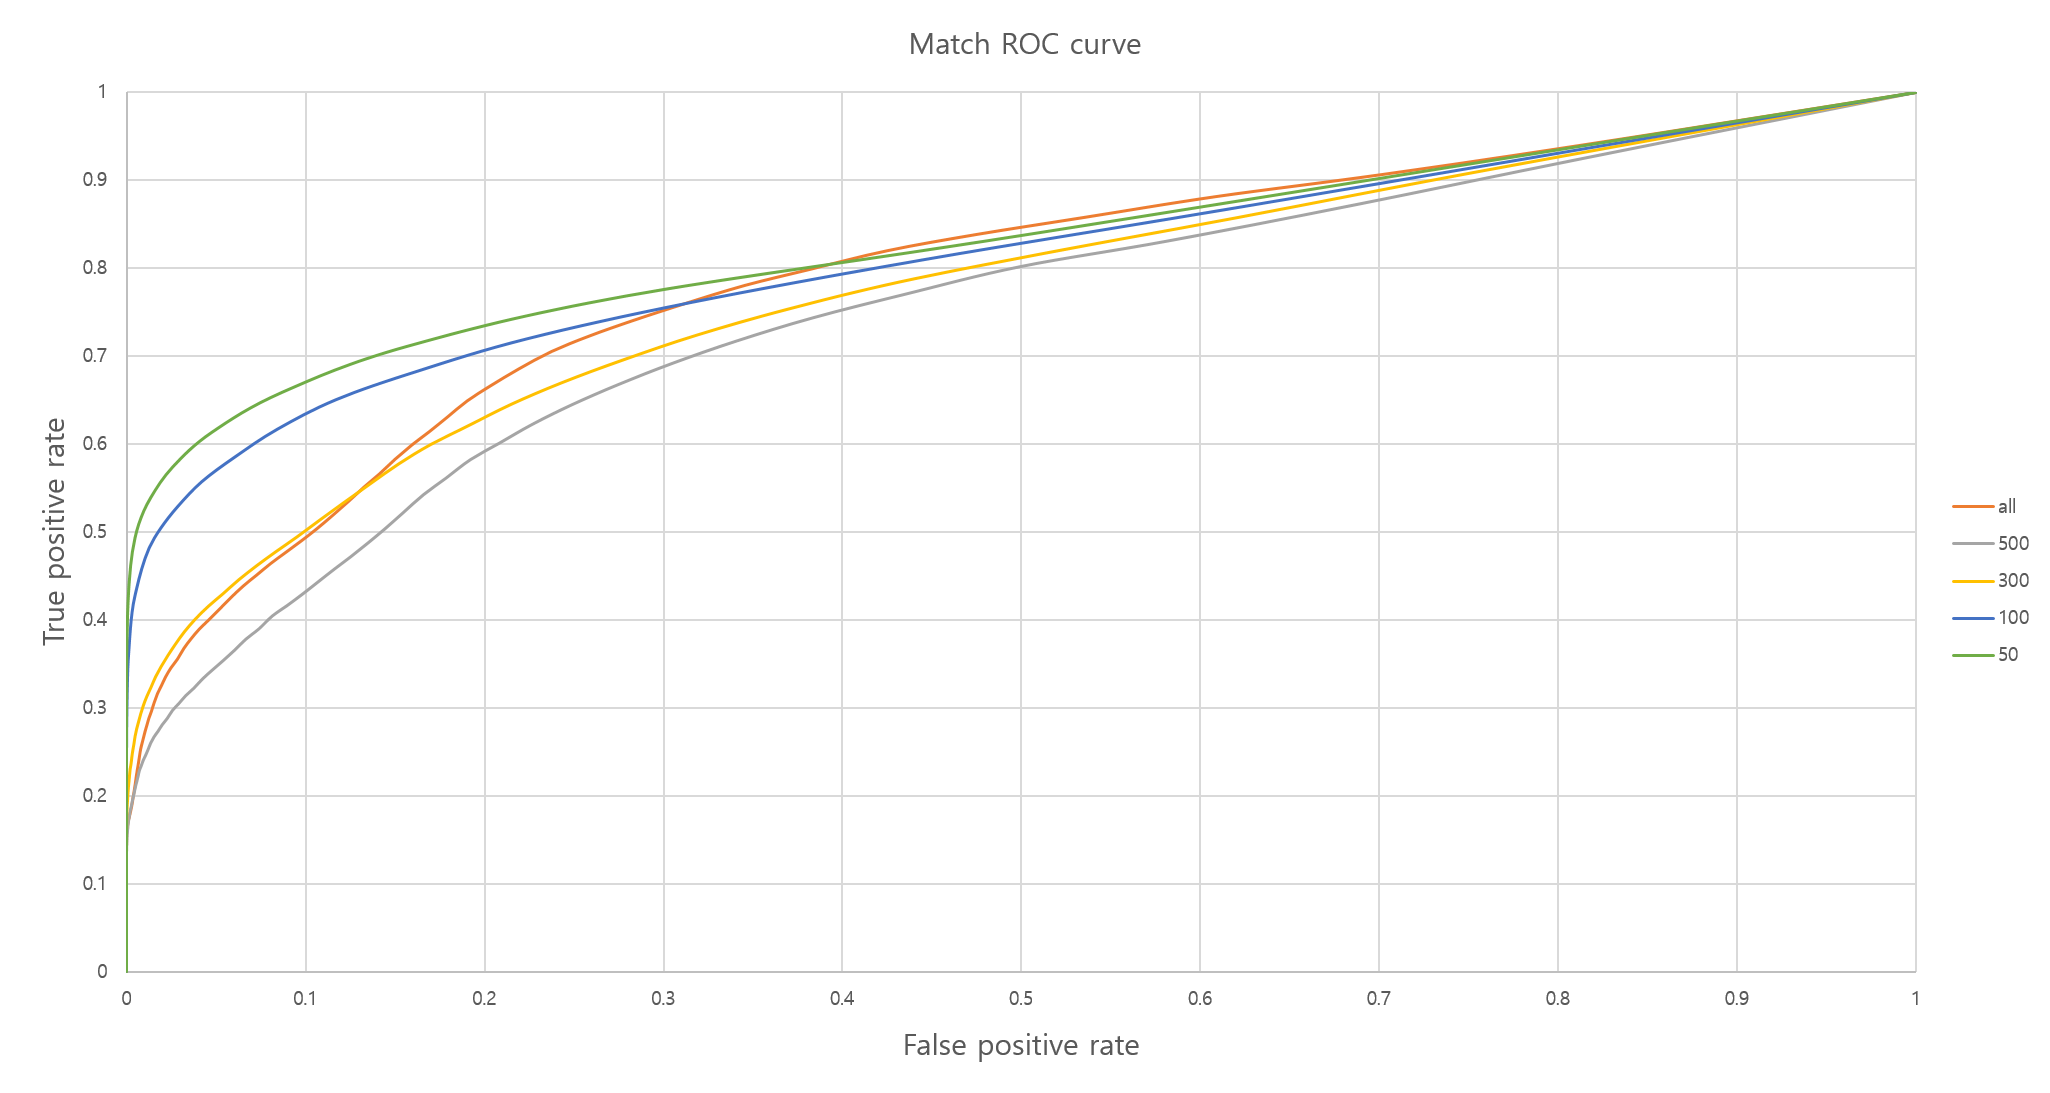
\includegraphics[width=1.0\columnwidth]{4_experiments/roc}
\caption{ROC curve for match rate}
\label{fig:markerless_roc}
\end{figure}

% 이러한 keypoint filtering을 수행하게 되면, miss-match를 유발하는 bad keypoint가 제거되기 때문에 match 결과의 reliability 가 높아진다. 이를 증명하기 위하여 Feature-level에서 Precision\cite{heinly_comparative_2012}을 계산하였다. Precision은 match 결과 구해진 correspondence pair의 수 대비 correct match의 비율로 계산이 된다. 이는 match 결과에 얼마나 miss-match가 적고 correct match의 비율이 높은지를 나타낸다. match 결과 대비 correct match의 비율이 높을수록 이후에 robust pose estimation의 성능에 영향을 미친다.

% When performing keypoint filtering, the bad keypoints causing miss-match are eliminated, which in turn increases the reliability of the match results. To prove this, the precision\cite{heinly_comparative_2012} in the feature-level was calculated. The precision can be calculated as the ratio between the number of the correspondence pairs obtained after matching and the correct matches, indicating the insignificant proportion of mass-match and significant proportion of correction match in the match results. The increase of the ratio between correct match and match results subsequently affects the performance of robust pose estimation. 


% % \begin{figure}[t!]
% % \centering
% % 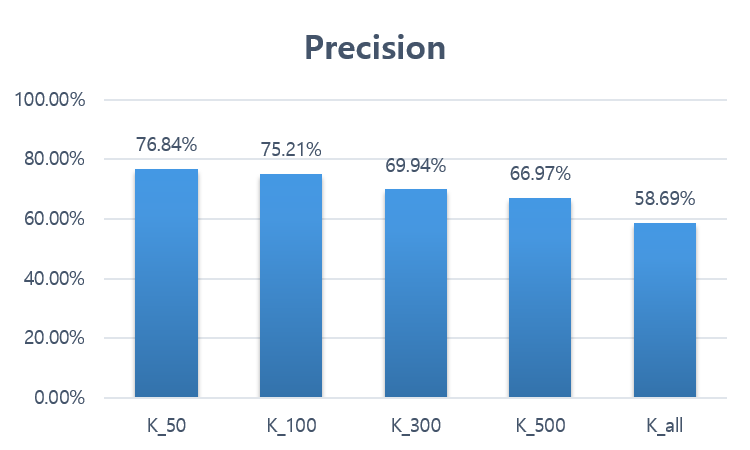
\includegraphics[width=1.0\columnwidth]{4_experiments/precision}
% % \caption{Precision of filtered keypoint database}
% % \label{fig:markerless_precision}
% % \end{figure}

% % \begin{table}[b!]
% % \centering
% % %\resizebox{\columnwidth}{!}{%
% % \begin{tabular}{llllll}
% % \hline
% % \textbf{}                   & \textbf{$K_{50}$} & \textbf{$K_{100}$} & \textbf{$K_{300}$} & \textbf{$K_{500}$} & \textbf{$K_{all}$} \\
% % \textbf{Avg. Match Result}  & 10.098            & 15.618             & 26.747             & 31.409             & 44.859             \\
% % \textbf{Avg. Correct Match} & 7.759             & 11.747             & 18.705             & 21.033             & 26.326             \\
% % \textbf{Precision}          & 76.8\%            & 75.2\%             & 69.9\%             & 67.0\%             & 58.7\%             \\ \hline
% % \end{tabular}
% % %}
% %   \caption{Precision of Filtered Matching}
% %   \label{tab:markerless_precision}
% % \end{table}

% % Precision의 결과는 그림 \ref{fig:markerless_precision}와 표\ref{tab:markerless_precision}에 나타난다. 전체 특징점 집합($K_{all}$)에 비하여 filtered 특징점 집합들이 더 높은 precision을 나타내주었다. 검출되는 특징점의 개수는 줄어들지만, Correct Match의 비율이 높아지기 때문에 높은 Precision을 보여주었다. 이러한 결과는 robst pose estimation의 속도와 성능을 향상시킬 수 있다.

% The results of precision are demonstrated in Table \ref{tab:markerless_precision} and Table \ref{fig:markerless_precision}. The filtered keypoints sets showed higher precision compared to the whole of keypoints set ($K_{all}$). The number of the detected keypoints decreased but the ratio of correct match increased, which showed high precision. Such results are able to improve the speed and performance of robust pose estimation.  

%!TEX root = ../icip_jseo.tex
% -*- root: ../icip_jseo.tex -*-

\section{Conclusion}

%본 논문에서는 Smart Space에서의 Seamless한 정보의 제공을 위하여 marker-less AR 기술을 개발하였다. Smart Space 환경에서는 Computing power가 제한적이기 때문에 이를 극복하기 위하여 경량화 된 marker-less AR 기술이 필요하다. 따라서 본 논문에서는 오프라인 학습 단계에서 detect된 특징점들을 평가하여 좋은 특징점만을 이용하여 학습하는 특징점 필터링 알고리즘을 제안하였다. 좋은 특징점은 영상의 변화에도 강인하게 detect되고, 자기 자신과의 매치 유사도가 높고, 다른 특징점과의 매치 유사도는 낮은 특징점을 의미한다. 이러한 특징을 반영하여 특징점을 filter 할 수 있는 score function을 정의하였다. 이를 통하여 offline train 단계에서 검출된 특징점을 filter 하여 저장함으로써, 전체적인 매치 연산을 줄여 속도를 향상시키면서도 영상의 인식율과 keypoint의 precision 을 높일 수 있었다.

% 로컬 키포인트 기반의 이미지 매칭 방법은 영상에서 특징이 되는 점(salient points)들의 특징을 저장하고 이를 실시간 영상과 매칭한다. 하지만,



In this paper, we propose a keypoint filtering approach to accomplish not only fast, but also robust and more reliable matching for mobile computing environment. Conventional keypoint matching methods rarely consider about quality of stored keypoint database. So, to accomplish robust matching quality, they require more keypoints. However, those redundant keypoints degrade matching quality. To overcome this problem, we evaluate detected keypoints and store only filtered keypoints. These filtered keypoints are repeatedly detected despite the change of images; show high match similarity with identical keypoints; and show low match similarity with other keypoints. Experimental results show that our filtering approach is effective in terms of both matching speed and quality thus applying this approach feasible for mobile image matching applications such as mobile object recognition or aumented reality.

% As a future work, we plan to apply this approach to other mobile applications and 

% 이 논문에서는 모바일 컴퓨팅 환경에서의 영상 매칭을 위하여 빠른 속도 뿐만이 아니라, 높은 인식율을 제공하는 새로운 키포인트 필터링 방법을 제안하였다. 기존의 키포인트 기반 매칭 방법은 키포인트의 품질에 대한 고려가 이루어지지 않고,반복이 잘 되는 점들을 저장하였다. 이에 따라서, 정확한 매칭 결과를 얻기 위해서는 많은 수의 키포인트가 필요하여 속도가 떨어질 뿐만 아니라, 질나쁜 키포인트로 인하여 false 매칭의 확률도 높았다. 본 논문에서는 이러한 방법을 극복하기 위하여 offline learning/training 단계에서 추출된 키포인트를 평가하여 매칭 성능이 높은 점들만 저장하는 방법을 제안한다. 







% In this paper, keypoints filtering algorithm, which used only the good keypoints selected after the evaluation the keypoints detected in the offline training phase, was proposed. 

% Good keypoints are rigidly detected despite the change of images; show high match similarity with themselves; and show low match similarity with other keypoints. The score function enabling it to filter the keypoints by reflecting above features was defined. It was possible to filter and save the keypoints detected in the offline training phase, which in turn increased the speed by reducing the overall match computation and thereby increased the precision of keypoints and the image recognition rate.  




% Below is an example of how to insert images. Delete the ``\vspace'' line,
% uncomment the preceding line ``\centerline...'' and replace ``imageX.ps''
% with a suitable PostScript file name.
% -------------------------------------------------------------------------
% \begin{figure}[htb]

% \begin{minipage}[b]{1.0\linewidth}
%   \centering
%   \centerline{\includegraphics[width=8.5cm]{image1}}
% %  \vspace{2.0cm}
%   \centerline{(a) Result 1}\medskip
% \end{minipage}
% %
% \begin{minipage}[b]{.48\linewidth}
%   \centering
%   \centerline{\includegraphics[width=4.0cm]{image3}}
% %  \vspace{1.5cm}
%   \centerline{(b) Results 3}\medskip
% \end{minipage}
% \hfill
% \begin{minipage}[b]{0.48\linewidth}
%   \centering
%   \centerline{\includegraphics[width=4.0cm]{image4}}
% %  \vspace{1.5cm}
%   \centerline{(c) Result 4}\medskip
% \end{minipage}
% %
% \caption{Example of placing a figure with experimental results.}
% \label{fig:res}
% %
% \end{figure}


% To start a new column (but not a new page) and help balance the last-page
% column length use \vfill\pagebreak.
% -------------------------------------------------------------------------
%\vfill
%\pagebreak


% References should be produced using the bibtex program from suitable
% BiBTeX files (here: strings, refs, manuals). The IEEEbib.bst bibliography
% style file from IEEE produces unsorted bibliography list.
% -------------------------------------------------------------------------
\bibliographystyle{IEEEbib}
% \bibliography{Remote}
\bibliography{reference}

\end{document}
